\documentclass[manuscript,review]{acmart}

%%% extra packages %%%
\usepackage{pifont}
\usepackage{algorithm}
\usepackage{algpseudocode}
\usepackage{tcolorbox}
\usepackage{float}


\title{Training a Generally Curious Agent}

%%% author section %%%
\author{Fahim Tajwar}
\authornote{Equal Contribution.}
\affiliation{%
    \institution{Carnegie Mellon University}
    \city{Pittsburgh}
    \country{USA}
}

\author{Yiding Jiang}
\authornotemark[1]
\affiliation{%
    \institution{Carnegie Mellon University}
    \city{Pittsburgh}
    \country{USA}
}

\author{Abitha Thankaraj}
\affiliation{%
    \institution{Carnegie Mellon University}
    \city{Pittsburgh}
    \country{USA}
}

\author{Sumaita Sadia Rahman}
\affiliation{%
    \institution{North Carolina State University}
    \city{Raleigh}
    \country{USA}
}

\author{J Zico Kolter}
\affiliation{%
    \institution{Carnegie Mellon University}
    \city{Pittsburgh}
    \country{USA}
}

\author{Jeff Schneider}
\affiliation{%
    \institution{Carnegie Mellon University}
    \city{Pittsburgh}
    \country{USA}
}

\author{Russ Salakhutdinov}
\affiliation{%
    \institution{Carnegie Mellon University}
    \city{Pittsburgh}
    \country{USA}
}

%%%% preamble %%%%
% removes the copyright/permission block
\setcopyright{none}

% removes "Manuscript submitted to ACM" footer
\settopmatter{printacmref=false}
\renewcommand\footnotetextcopyrightpermission[1]{}

% removes "Authors' Contact Information" block
\authorsaddresses{}

\pagestyle{plain}
\fancyfoot{}

% collect leftover vertical space at the bottom of pages instead of stretching
% the gaps between table/text in the middle
\raggedbottom

\begin{document}

% %%% footnote that was in the paper %%%
% \begingroup\renewcommand\thefootnote{}\footnotetext{%
% Proceedings of the 42\textsuperscript{nd} International Conference on Machine Learning, 
% Vancouver, Canada. PMLR 267, 2025. Copyright 2025 by the author(s).%
% }\endgroup

\begin{abstract}
{
Efficient exploration is essential for intelligent systems interacting with their
environment, but existing language models often fall short in scenarios that require
strategic information gathering. In this paper, we present \textsc{PAPRIKA}, a fine-tuning
approach that enables language models to develop general decision-making capabilities that
are not confined to particular environments. By training on synthetic interaction data
from different tasks that require diverse strategies, \textsc{PAPRIKA} teaches models
to explore and adapt their behavior on a new task based on environment feedback
in-context without more gradient updates. Experimental results shows that models 
fine-tuned with \textsc{PAPRIKA} can effectively transfer their learned decision-making
capabilities to entirely unseen tasks without additional training. Unlike traditional
training, our approach's primary bottleneck lies in sampling useful interaction data
instead of model updates. To improve samples efficiency, we propose a curriculum 
learning strategy that prioritizes sampling trajectories from tasks with high learning
potenti. To improve samples efficiency, we propose a curriculum 
learning strategy that prioritizes sampling trajectories from tasks with high learning
potential. These results suggest a promising path towards AI systems that can autonomously
solve novel sequential decision-making problems that require interactions with the external
world.
}
\end{abstract}


\maketitle

%%%%%%%%%%%%%%%%%%%%%%%%%%%%%%%%%%%%%%%%%%%%%%%%%%%%%%%%%%%%%%%%
\section{Introduction}
{
Large Language Models (LLMs) are the backbone for autonomous agents, systems capable of
achieving goals independently with minimal human supervision or intervention. Being interactive
and exploratory is a crucial part of completing its objectives. However, two challenges limit these
interactive capabilities. Firstly, naturally occuring tasks and data are unstructured and 
lack the structure needed to guide smooth model interactions. Second, directly deploying models
into the real world to collect interaction data can produce critical errors.

Using \emph{in-context learning} (ICL), LLMS can be trained on synthetic data, that allows
them to adapt to tasks with minimal demonstrations\cite{brown2020language}. The model
can also be taught \emph{in-context reinforcement learning}\cite{laskin2022context}.
In this way, the model learns the general method to solve new problems, instead of being
fed raw data. This paradigm shares similarities to supervised fine-tuning (SFT) and reinforcement
learning from human feedback (RLHF) stages of training a language model (vs pretraining) where
only a relatively small number of examples is needed to produce a model that can generate
responses to a wide range of queries that it is not trained on. 
This approach also closely follows the principles of \emph{meta reinforcement learning}
\cite{beck2023survey}. Another popular notion of motivation is \emph{intrinsic motivation}
\cite{schmidhuber1991curious}. Our work differs from this notion of curiosity 
in that we do not leverage any intrinsic motivation, 
rather we train our agents to explore and interact with an
entirely unseen environment to gather required information that is needed for
completing the task at hand. \textsc{PAPRIKA} can be thought of as a from of
amortized exploration, since the main goal is to learn good exploration strategies from 
trajectories from many different environments on a new problem.

Using a base model, we generate interaction trajectories and assign scores
based on their success in achieving the tasks' objectives. We then apply a sequential 
variant of Direct Preference Optimization\cite{rafailov2024direct} to increase the 
likelihood of successful trajectories. Our approach's primary bottleneck lies in
sampling useful interaction data and not computational costs. As such, a curriculum 
learning strategy was introduced. We refer to the overall framework as \textsc{PAPRIKA 
\footnote{The name is inspired by the movie "Paprika" (2006), where a dream detective navigates vast and strange dream worlds to solve different mysteries.}}.
It highlights in-context RL using synthetic data rather than traditional costly
task-specific training.

% i can reference it in the text with Figure~\ref{fig:paprika}
\begin{figure}[t]
    \centering
    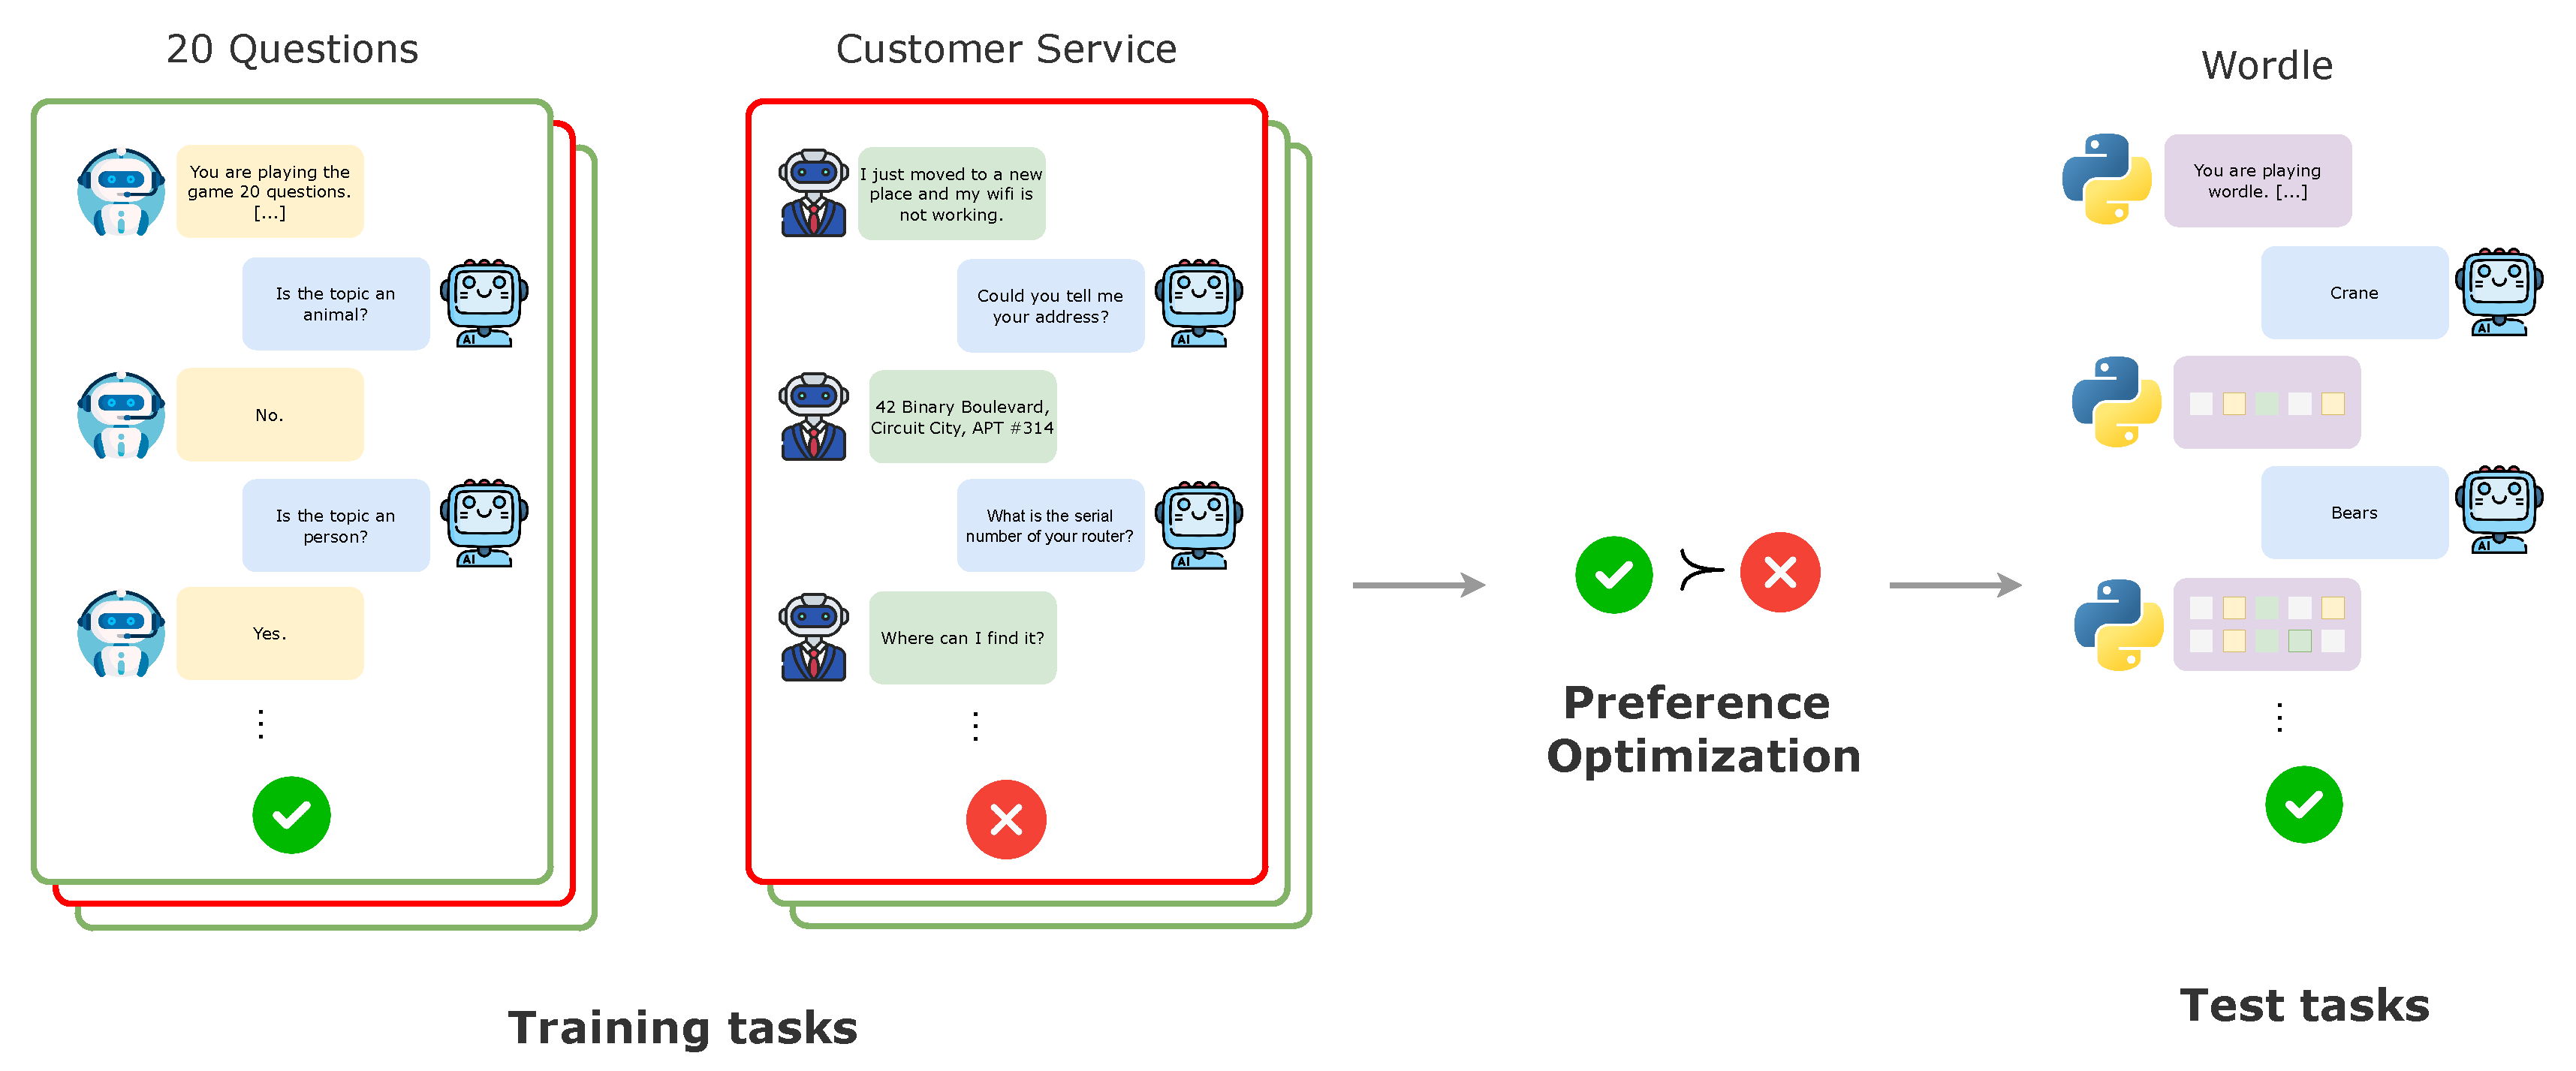
\includegraphics[width=0.85\linewidth]{figures/paprika-fig1-v2.pdf}
    \Description{Overview diagram of the \textsc{PAPRIKA} framework showing task generation,
    trajectory scoring, and training to prefer higher-performing trajectories for
    zero-shot transfer to unseen tasks.}
    \caption{\textbf{(Overview of \textsc{PAPRIKA})}}
    A diverse set of tasks where an LLM agent needs strategic information 
    gathering to succeed are designed, then an LLM is trained on self-generated data
    to prefer higher performing trajectories. The resulting behavior learned by
    \textsc{PAPRIKA} can transfer zero-shot to unseen tasks, showcasing its potential 
    to build general decision making agents.
    \label{fig: paprika}
\end{figure}
}

%%%%%%%%%%%%%%%%%%%%%%%%%%%%%%%%%%%%%%%%%%%%%%%%%%%%%%%%%%%%%%%%
\section{Related Works}
{
\paragraph{LLM alignment.} { 
Alignment or post-training is a crucial step for creating a helpful LLM assistant.
Typically, RLHF pipelines\cite{christiano2017deep} work best. We focus on the multi-turn settings
where the agent has to interact with an environment iteratively, similar to
\cite{rafailov2024rqlanguagemodel}. There are many existing environments and
dataset focusing on multi-turn interactions, most of which focus on interactions 
with humans. Rather than a particular task, we focus on evaluating LLM's general
ability to solve sequential decision making problems where the agent needs to 
explore and exploit.
}

\paragraph{In-context reinforcement learning.}{
In-context learning (ICL) is the ability where LLMs can learn a new task from a small
number of demonstrations without gradient updates\cite{brown2020language}. Exsiting
ICL focuses on single-turn interaction. We focus on in-context reinforcement learning
\citep{laskin2022context, raparthy2023generalization, lee2024supervised, lin2024transformers}.
We mainly focus on diverse environments and study how well the decision making abilities
generalize to completely new environments.
}

\paragraph{Curriculum learning in RL.} {
Curriculum learning\cite{bengio2009curriculum} shows the data to the model in a 
non-uniform order, inspired by the fact that humans tend to learn things in a 
sequential order\cite{skinner1958reinforcement} and is particularly appealing for 
RL because learning easier tasks first could build scaffold toward solving difficult
tasks that the agent could not solve otherwise\cite{andrychowicz2017hindsight,florensa2017reverse,fang2019curriculum}.
Concurrent works\cite{foster2025learningreasonfrontierlearnability} has studied
curriculum learning extensively for training LLMs particularly to improve reasoning.
Given grouping metadata, effective curriculum learning can be designed.
}

%%% preliminaries / notation %%%
\section{Preliminaries}{
Many decision making problems can be formalized as a partially observable Markov decision process (POMDP), 
and we assume each \emph{task} $\tau$ to be a POMDP,

A \emph{group} (or task group, used interchangeably), $$G = \{\tau_1, \tau_2, \dots, \tau_{|G|}\}$$ 
is a high-level grouping of tasks that share similar strategies. For example,
the game twenty questions is a group, and guessing the word ``\texttt{apple}'' is one task in it. 
From the agent's perspective, each task is a black box that takes the agent's action $a_t$ and 
outputs an observation $o_t$, both of which are strings. 

An episode, $$h = (o_0, a_0, \dots, o_H, a_H)$$ is the
agent's interaction trajectory within a single task, with $h_{p:q}$ denoting a slice of it
similar to array slicing. An episode terminates when the agent achieves the objective or
the maximum number of allowed interactions is reached, at which point the environment
emits a single score $r(h)$.

Let $\pi$ denote the LLM agent and $h \sim \pi \circ \tau$
denote sampling a trajectory from task $\tau$ using policy $\pi$. The performance of a
policy on a group is
\begin{equation}
    \texttt{Perf}(G) = \frac{1}{|G|}\sum_{\tau \in G} \mathbb{E}_{h\sim \pi \circ \tau}[r(h)].
\end{equation}
The agent is trained on a finite set of groups $\mathcal{G}_\text{train}$, and the goal is
to perform well on unseen groups $\mathcal{G}_\text{test}$.
}
}
%%%%%%%%%%%%%%%%%%%%%%%%%%%%%%%%%%%%%%%%%%%%%%%%%%%%%%%%%%%%%%%%
\section{Method}
{
Prior works have shown that LLMs can perform poorly even on the simple decision making
task of multi-armed bandits\cite{krishnamurthy2024largelanguagemodelsexplore}, and that
fine-tuning on synthetic trajectories generated by known algorithms such as UCB can teach
them to do better\cite{nie2024evolveevaluatingoptimizingllms}. However, this idea is
limited in scope: we want LLMs to explore strategically in far more complex settings,
for most tasks there is no known algorithm like UCB to generate good trajectories from,
and it is infeasible to collect data for every task we care about. \textsc{PAPRIKA}
solves these issues in steps. First, a suite of complex decision-making tasks requiring
strategic information gathering is designed. Next, in the absence of known good algorithms,
existing LLMs generate trajectories with better decision making behaviors through
diversity-encouraging sampling. The LLM is then fine-tuned to prefer higher performing
trajectories, in a fashion similar to STaR\cite{zelikman2022starbootstrappingreasoningreasoning},
and these behaviors often generalize to unseen task groups without additional training.
Finally, a curriculum learning algorithm dynamically chooses which subset of tasks to
train on next to improve data efficiency.

\subsection{Task Design}
{
The task groups should have four desired properties: \textbf{(1)} they are purely text
based, \textbf{(2)} they require multi-turn interaction, where the agent has to understand
prior history in its context and choose actions that maximize the probability of future
success, \textbf{(3)} they are partially observable, so the agent must simultaneously
explore to reveal more information and exploit to solve the task efficiently, and
\textbf{(4)} they are diverse and require different strategies to succeed. With these
requirements in mind, 10 task groups are designed, summarized in
Table~\ref{tab:environment_summary}. 

In all of them, an LLM agent solves a task through
sequential interaction with the task-specific environment, which provides both
intermediate observations and a task reward at the end of an episode.

%%% table 1: task group summary %%%
\begin{table}
    \caption{Summary of the task groups used by \textsc{PAPRIKA}.}
    \label{tab:environment_summary}
    \centering
    \begin{tabular}{c|c c c c c}
    \toprule
        Task Group  & \# Train Tasks & \# Test Tasks & Maximum Turns & Env Feedback & Uses COT \\
        \midrule
         Twenty questions           & 1499  & 367 & 20  & LLM generated     & \ding{55}     \\
         Guess my city              & 500   & 185 & 20  & LLM generated     & \ding{55}     \\
         Wordle                     & 1515  & 800 & 6   & Hardcoded program & \checkmark    \\
         Cellular automata          & 1000  & 500 & 6   & Hardcoded program & \checkmark    \\
         Customer service           & 628   & 200 & 20  & LLM generated     & \ding{55}     \\
         Murder mystery             & 203   & 50  & 20  & LLM generated     & \ding{55}     \\
         Mastermind                 & 1000  & 500 & 12  & Hardcoded program & \checkmark    \\
         Battleship                 & 1000  & 200 & 20  & Hardcoded program & \checkmark    \\
         Minesweeper                & 1000  & 200 & 20  & Hardcoded program & \checkmark    \\
         Bandit best arm selection  & 81    & 1   & 21  & Hardcoded program & \checkmark    \\
         \bottomrule
    \end{tabular}
\end{table}

Following prior work\cite{abdulhai2023lmrl}, classic guessing games like
\textit{twenty questions} and \textit{guess my city} are included, which require guessing
a secret topic as quickly as possible by asking a sequence of questions. In \textit{Wordle}
and \textit{Mastermind}, the agent needs to guess a secret 5-letter word and 4-digit code
respectively, where the environment gives feedback about the similarity between the guess
and the target, and the agent must refine its future guesses accordingly.

\textit{Customer service} and \textit{murder mystery} are dynamic text-based groups: an
LLM plays the role of the environment and generates intermediate observations based on a
given success criterion. \textit{Cellular automata} simulates coding against interpreter
feedback in a toy setting, where the agent makes inferences about the transition rule of
a 1D elementary cellular automaton by observing inputs and outputs.
\textit{Minesweeper} and \textit{Battleship} require interacting with 2D grids to find
hidden items within a fixed number of turns.

Finally, a modified version of the
multi-armed bandit group is included, where the agent works on the \textit{bandit best
arm selection} problem with the following distinctions: (1) we let the agent employ
Chain of Thought Reasoning (CoT) before choosing arms so that they can transfer good
strategies learned from the other tasks, (2) we let the agent interact with the task
environment in a multiturn way, (3) and the agent has the ability to choose arms and
observe rewards for a fixed number of turns and then measure its accuracy in deciding
the arm with the highest reward, instead of reducing regret. This reduces computational
cost over generating COTs for a large number of turns, since the difference in regret between
different models is not meaningful when the number of turns is not large enough.

For tasks requiring general knowledge about the world, another LLM (typically GPT-4o-mini)
is employed as the environment, while tasks with rule-based observations and rewards use
hardcoded programs, which are more reliable than
LLMs\cite{deepseekai2025deepseekr1incentivizingreasoningcapability}. To prevent reward
hacking, another LLM or a hardcoded program is used as a judge to filter out unsuccessful
trajectories that got incorrectly labeled as successful. For task groups requiring complex
reasoning, letting the agent think using chain-of-thought (COT) prompting\cite{wei2022chain}
before generating a final answer improves performance significantly, similar to
ReAct\cite{yao2023reactsynergizingreasoningacting}.

%%% example task environments %%%
As an example of a task group with an LLM-simulated environment,
Figure~\ref{fig:twenty_questions_prompt} shows the first user prompt received by the
agent playing twenty questions, containing general instructions about the task and the
type of hidden topic it needs to guess.

\begin{figure}[H]
\begin{tcolorbox}[colback=gray!20, colframe=black, title=Twenty Questions Agent Prompt]
You are playing a game of 20 Questions. Your goal is to guess the name of a thing or
person by asking up to 20 yes-or-no questions. After each question, you will receive an
answer: `Yes' or `No.' Use the answers provided to refine your guesses.

Here are your instructions:

- You can ask only yes-or-no questions.

- After receiving each answer, you should adapt your questions based on the new information.

- Your goal is to guess the topic in as few questions as possible.

- If you're confident, you can make a guess before reaching 20 questions.

The game starts now. You are trying to guess a clothing. Ask your first question!
\end{tcolorbox}
\Description{Example first user prompt given to the agent in the twenty questions task group.}
\caption{Example agent prompt for the twenty questions task group, where the environment
is simulated by another LLM.}
\label{fig:twenty_questions_prompt}
\end{figure}

The environment here is another LLM that receives the secret topic and answers the
agent's questions strictly with `Yes', `No', or `Goal reached'. In contrast, task groups
like wordle use a hardcoded program as the environment:
Figure~\ref{fig:wordle_feedback} shows the observation the program generates given the
secret word ``toast'' and the agent's guess ``boost''.

\begin{figure}[H]
\begin{tcolorbox}[colback=gray!20, colframe=black, title=Wordle Task Environment Feedback]
First letter, b, is not in the target word

Second letter, o, is correct and in the correct position in the target word

Third letter, o, exists in the target word but in a different position

Fourth letter, s, is correct and in the correct position in the target word

Fifth letter, t, is correct and in the correct position in the target word

Make your next guess about the hidden word. Please try to be concise. Format your
response in the following way: \texttt{<Think>} Any step-by-step, short and concise
thinking to strategically determine the next guess for the secret word \texttt{</Think>}

\texttt{<Answer>} your guess of what the word should be \texttt{</Answer>}
\end{tcolorbox}
\Description{Example per-letter feedback generated by the hardcoded wordle environment.}
\caption{Example environment feedback for the wordle task group, generated by a
hardcoded program.}
\label{fig:wordle_feedback}
\end{figure}
}

\subsection{Dataset Construction}
{
The data generated from these task groups must be diverse, which allows the model to
learn different strategies without the risk of overfitting. This is accomplished by
generating a large number of trajectories at a high temperature with Min-p
sampling\cite{nguyen2024turning}. Min-p sampling uses an adaptive threshold
$p_\text{scaled} \propto p_\text{max}$, where $p_\text{max}$ is the highest probability
predicted by the model on the next token, and truncates the vocabulary to tokens with
probability larger than $p_\text{scaled}$ --- this keeps the trajectories coherent even
at higher temperatures. For each chosen task, $n_\text{sample}$ trajectories are generated
and a preference pair $(h_{w}, h_{l})$ is constructed, where $h_{w}$ is the highest
scoring trajectory (succeeds at the fewest number of turns) and $h_{l}$ is sampled
randomly from the lower scoring trajectories instead of the worst one, in order to
increase the diversity of the dataset. These act as proxies for desirable and undesirable
behaviors. A dataset $\mathcal{D} = \left\{\left(h^{w}, h^{l}\right)^{(i)}\right\}_{i=1}^N$
is a collection of such trajectory pairs.
}

\subsection{Optimization}
{
\paragraph{Supervised fine-tuning.}{
If the winning episodes are taken as expert behavior, the losing episodes can be discarded
and the likelihood of the winning ones maximized:
\begin{align}
    \label{eq:sft}
    \mathcal{L}_\text{SFT}(\mathcal{D}_\text{SFT}) = -\mathbb{E}_{\mathcal{D}_\text{SFT}} \left[ \frac{1}{\sum_{t=0}^{|h_w|}|a_t^w|}\sum_{t=0}^{|h_w|} \log \pi_\theta \left(a^w_t \mid h^w_{:t}\right) \right]
\end{align}
where $\mathcal{D}_\text{SFT}$ is the dataset used for supervised fine-tuning and $|a|$
is the number of tokens of the agent response, discarding the environment generation.
}

\paragraph{Direct preference optimization.}{
DPO\cite{rafailov2024direct} directly optimizes the Bradley-Terry
model\cite{bradley1952rank} for preferences. In this setting each trajectory consists of
multiple rounds of interaction, so the original DPO objective does not apply, and a
multi-turn version\cite{rafailov2024rqlanguagemodel} is used instead:
\begin{equation}
    \mathcal{L}_{\text{DPO}}\left( \mathcal{D}_{\text(DPO)} \right) = -\mathbb{E}_{ \mathcal{D}_{\text{DPO}} } \left[ \log \sigma \left( \sum_{t = 0}^{|h^w|} \beta \log{\dfrac{\pi_{\theta} \left( a_{t}^{w} | h_{:t}^{w} \right)}{\pi_{\text{ref}} \left( a_{t}^{w} | h_{:t}^{w} \right)}} - \sum_{t=0}^{|h^t|} \beta \log{ \dfrac{ \pi_{\theta} \left( a_{t}^{l} | h_{:t}^{l} \right) }{ \pi_{\text{ref}} \left( a_{t}^{l} | h_{:t}^{l} \right) } } \right) \right]
\end{equation}
where $\mathcal{D}_\text{DPO}$ is the preference dataset, $a_t^w$ and $a_t^l$ are the
action tokens generated by the model at turn $t$ in the preferred and dispreferred
trajectories $h^w$ and $h^l$, and $\pi_\text{ref}$ is the reference policy, taken to be
the initial model. The main difference with standard DPO is that the loss is calculated
only on the action tokens --- the log probability ratios of the environment generated
tokens are not included. DPO is chosen because it is less compute intensive and allows
decoupling the data collection and policy improvement steps, though online RL with more
resources would be expected to give even stronger results.
}

\paragraph{Combining objectives.}{
DPO can have the unintended effect of reducing the probability of the preferred
trajectories as well, known as unintentional
unalignment\cite{razin2024unintentionalunalignmentlikelihooddisplacement}. The RPO
objective\cite{pang2024iterativereasoningpreferenceoptimization} mitigates this issue by
combining the SFT and DPO losses:
\begin{equation}
    \label{eq:rpo}
    \mathcal{L}_{\text{RPO}}(\mathcal{D}_\text{DPO}) = \mathcal{L}_\text{DPO}(\mathcal{D}_\text{DPO}) + \alpha \mathcal{L}_\text{SFT}(\mathcal{D}_\text{DPO})
\end{equation}
where $\alpha$ is a hyper-parameter, set to 1.0 for the rest of the paper.
}
}

\subsection{Scalable Online Learning Curriculum}
{
It is relatively easy to design a large number of tasks, but harder to decide which ones
to train on. If a task is too difficult for the current model, the generated trajectories
carry no meaningful learning signal, and since generating trajectories is the dominant
cost of training, tasks where the model can make meaningful progress should be
prioritized --- a form of curriculum learning\cite{bengio2009curriculum}. The only way to
know whether a task yields good learning signal is to actually perform rollouts on it,
which is expensive, so an efficient curriculum must predict this without the rollout. A
natural assumption is that similar tasks have similar levels of learning signal, and such
groupings can be obtained through metadata or prior knowledge.

\paragraph{Measuring learning potential.}{
The average performance of $\pi$ on $\tau$ is
$R_\pi(\tau) = \mathbb{E}_{h \sim \pi \circ \tau }\left[r(h)\right]$ and the variance is
$\sigma^2_\pi(\tau) = \mathbb{E}_{h \sim \pi \circ \tau }\left[(r(h) - R_\pi(\tau))^2\right]$.
Based on these, the learning potential of a single task is defined as
\begin{align}
\label{eq:nu}
    \nu_\pi(\tau) = \frac{\sqrt{\sigma^2_\pi(\tau)}}{R_\pi(\tau)}.
\end{align}
This quantity is known as the coefficient of variation in statistics, a dimensionless
quantity that measures the population's variability relative to the mean. Variance
naturally measures the possibility of getting diverse trajectories from sampling, which
matters because DPO suffers when the preferred and dispreferred responses are not
sufficiently different\cite{pal2024smaugfixingfailuremodes}. On the other hand, different
tasks can have vastly different reward scales, and normalizing the standard deviation
by the mean allows comparing different tasks directly.
}

\paragraph{Sampling tasks.}{
Since it is infeasible to evaluate $\nu_\pi(\tau)$ for all tasks, tasks are sampled from
each group instead. Given a collection of $K$ groups, choosing which group to sample from
next to maximize learning potential can be formulated as a multi-armed bandit problem,
solved here with the Upper Confidence Bound (UCB) algorithm\cite{auer2000using}. Each
action corresponds to a group of tasks: one task is sampled uniformly from the chosen
group, the model is evaluated on it with $C$ rollouts, and these statistics update the
mean estimate of that group. After a sufficient number of episodes are sampled, the
dataset is constructed and the model is trained with the objectives above.
Algorithm~\ref{alg:sampling} shows the pseudocode.
}

%%% algorithm 1: task selection with ucb %%%
\begin{algorithm}[t]
\caption{Task selection with UCB}
\label{alg:sampling}
\begin{algorithmic}[1]
\State \textbf{Input:} Number of arms $K$, number of samples $C$, number of rounds $T$, model $\pi$
\State \textbf{Initialize:} $s_k=0$, $n_k=0$, \texttt{Buffer}
\For{each round $t = 1, 2, \dots, T$}
    \State Compute $\theta_k = \tfrac{s_k}{n_k} + \sqrt{\tfrac{2 \log \sum_{k=1}^K n_k}{n_k}}$ for each $k$
    \State Select $k^\star = \arg\max_k \theta_k$
    \State Sample $\tau$ from group $k^\star$
    \State Sample $C$ trajectories from $\tau$ and add to \texttt{Buffer}
    \State Compute an estimate for $\hat{\nu}_\pi(\tau)$ using Eq~\ref{eq:nu}
    \State Update: $s_{k^\star} = s_{k^\star} + \hat{\nu}_\pi(\tau), \, n_{k^\star} = n_{k^\star} + 1$
\EndFor
\State Construct $\mathcal{D}$ from \texttt{Buffer} and train the model $\pi$
\end{algorithmic}
\end{algorithm}
}
}

%%%%%%%%%%%%%%%%%%%%%%%%%%%%%%%%%%%%%%%%%%%%%%%%%%%%%%%%%%%%%%%%
\section{Results}
{
The empirical study answers the following research questions: \textbf{(1)} Can training
on self-generated trajectories from a diverse range of task groups equip LLMs with
sequential decision making capabilities that generalize to unseen task groups without
training on them? \textbf{(2)} Can curriculum learning improve the data efficiency of
this training mechanism? \textbf{(3)} Does \textsc{PAPRIKA} hurt the model's regular
abilities?

\paragraph{Experimental setup.}{
Llama-3.1-8B-Instruct\cite{grattafiori2024llama3herdmodels} and
Gemma-3-12B-IT\cite{gemmateam2025gemma3technicalreport} models are used for all
experiments. Training data is generated with Min-p sampling at temperature 1.5 and Min-p
parameter 0.3, which consistently produced diverse data resulting in higher test-time
accuracy. For each task in the training split, $n_\text{sample} = 20$ trajectories are
generated (100 for mastermind), which after filtering results in 17,181 training
trajectories for supervised fine-tuning and 5,260 trajectory pairs for RPO over all task
groups. The learning rate is $10^{-6}$ for supervised fine-tuning and $2 \times 10^{-7}$
for RPO with batch size 32, using an AdamW
optimizer\cite{loshchilov2019decoupledweightdecayregularization} with a cosine annealing
schedule and warmup ratio 0.04\cite{loshchilov2017sgdrstochasticgradientdescent}.
Supervised fine-tuning is always run first, followed by further fine-tuning with the RPO
objective. During evaluation, 4 trajectories are generated for each task in the test set
with Min-p parameter 0.3 at temperature 0.7, and the average success rate is reported.
For task groups with hardcoded feedback, a failure to follow formatting instructions
counts as a failure in the task.
}

\paragraph{\textsc{PAPRIKA} improves LLM decision making abilities.}{
The toy group of bandit best arm selection requires strategic use of a fixed sampling
budget to quickly discard unpromising arms. While previous work improved LLMs on bandits
by training on trajectories from optimal bandit algorithms, \textsc{PAPRIKA} improves
the average success rate of Llama-3.1-8B-Instruct on this group from 42.25\% to 62.25\%
after only seeing trajectories from \emph{other} task groups, without needing any optimal
algorithm to generate synthetic data. On the full suite,
Figure~\ref{fig:paprika_success_rate} shows that training on filtered trajectories from
all 10 task groups improves the success rate of both models. Averaged across all groups,
\textsc{PAPRIKA} increases the Llama model's performance by 47\% of its original success
rate after training on only about 22,500 trajectories.
}

%%% figure 2: success rate on all 10 task groups %%%
\begin{figure}[t]
    \centering
    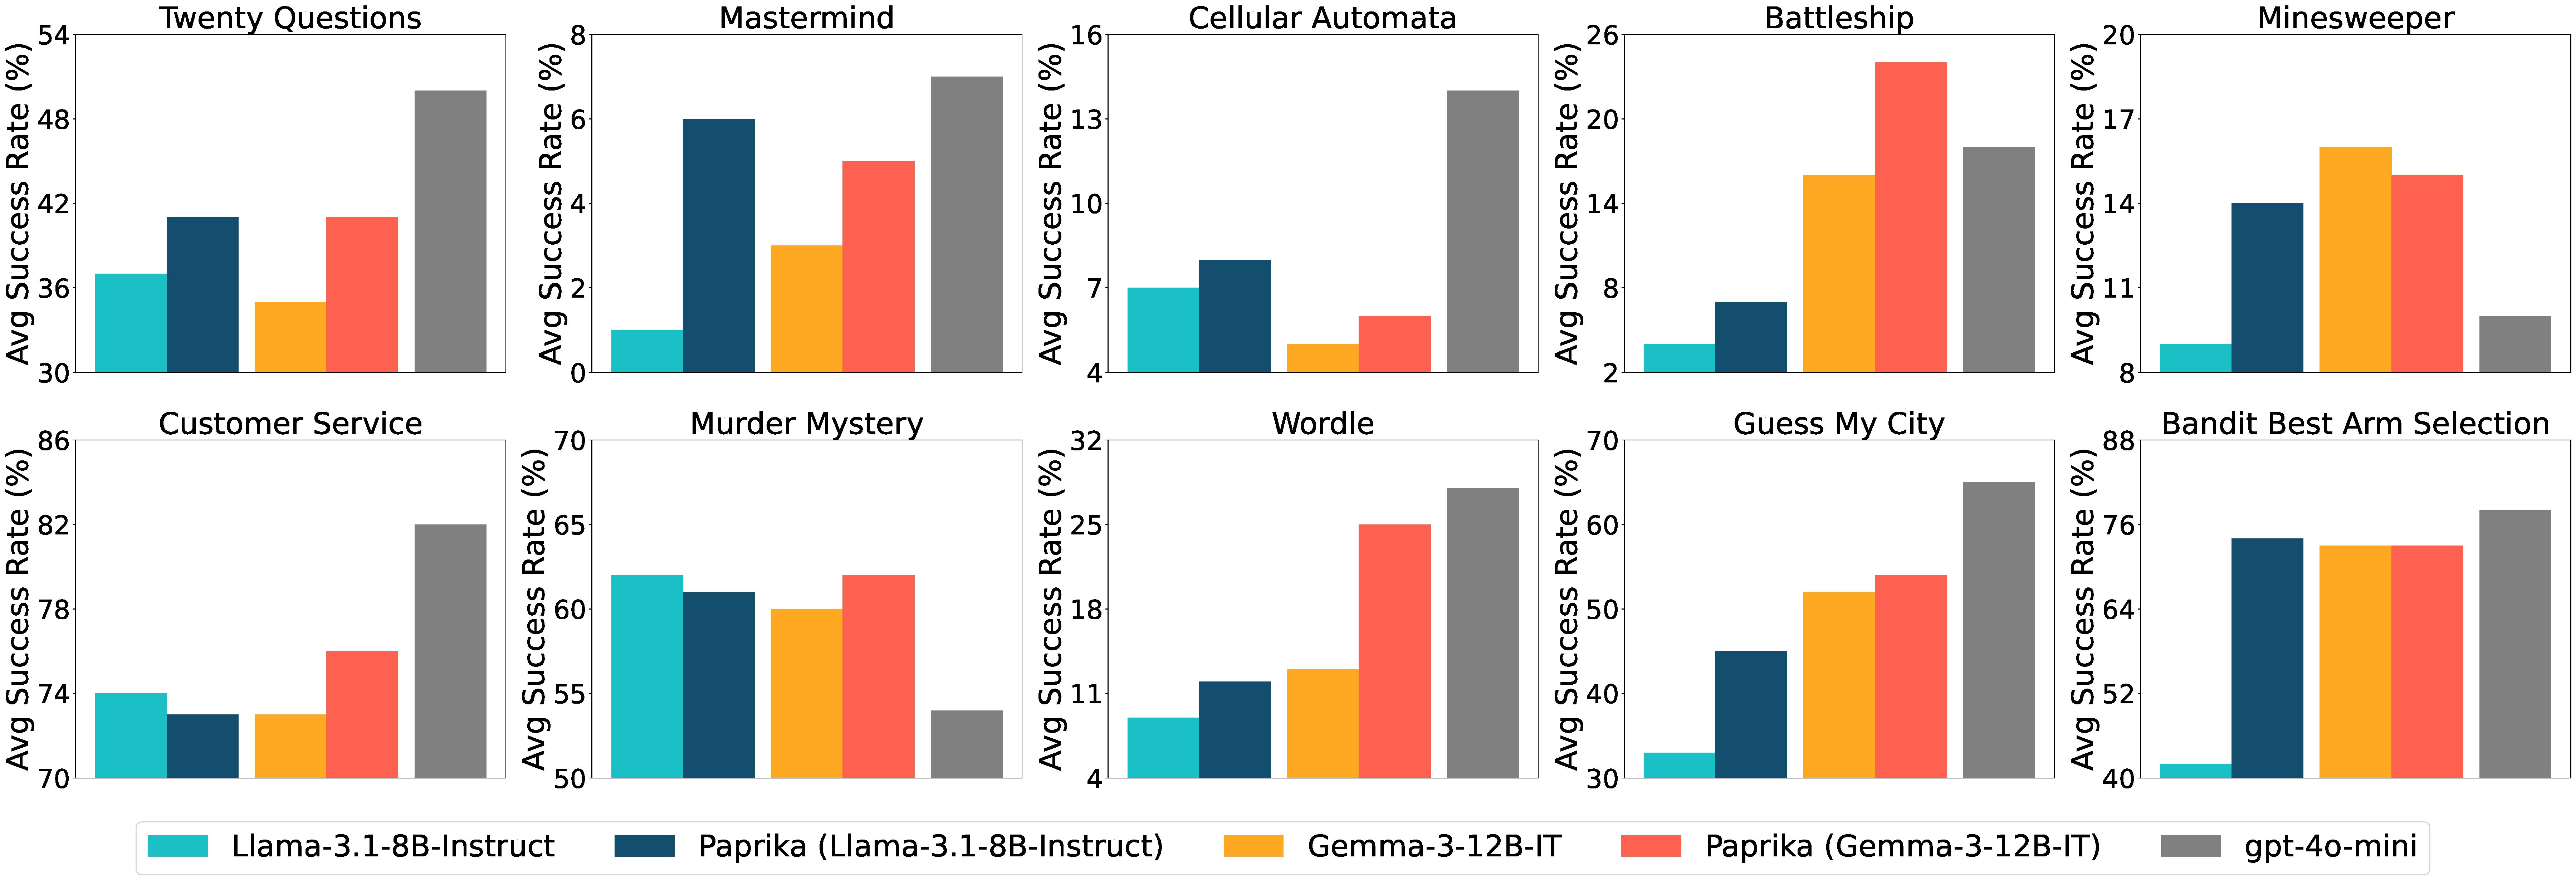
\includegraphics[width=0.95\linewidth]{figures/relative_improvement_in_success_rate.pdf}
    \Description{Bar chart of average success rates on all 10 task groups, comparing the
    base models against their PAPRIKA fine-tuned versions.}
    \caption{\textbf{(\textsc{PAPRIKA} improves success rate on a diverse range of task
    groups)} 
    Average success rate on all 10 task groups at temperature 0.7.
    \textsc{PAPRIKA} generally improves performance of both Llama-3.1-8B-Instruct and
    Gemma-3-12B-IT models.}
    \label{fig:paprika_success_rate}
\end{figure}

\paragraph{\textsc{PAPRIKA} can teach LLMs generalizable strategies.}{
To study whether the learned strategies zero-shot transfer to entirely different groups,
a set of leave-one-out (LOO) experiments is performed: one group is chosen, the LLM is
trained on trajectories from every other group, and the resulting model is tested on the
left-out group. Additionally, for each group a model is trained and tested on that single
group alone. Figure~\ref{fig:generalization_leave_one_out_experiments} shows the results:
the LOO models can match or sometimes even exceed the performance of group-specific
training, improving success rate on 9 out of 10 task groups compared to the initial
model. Moreover, \textsc{PAPRIKA} trained on all 10 groups outperforms single-group
training on 7 out of 10 groups, showing that the model learns better in-group strategies
when it observes trajectories from other groups. The transfer is not universal --- the
improvement on mastermind is minimal and wordle shows negative transfer --- but scaling
up the number of task groups could keep improving zero-shot decision-making abilities.
}

%%% figure 3: leave-one-out generalization %%%
\begin{figure}[t]
    \centering
    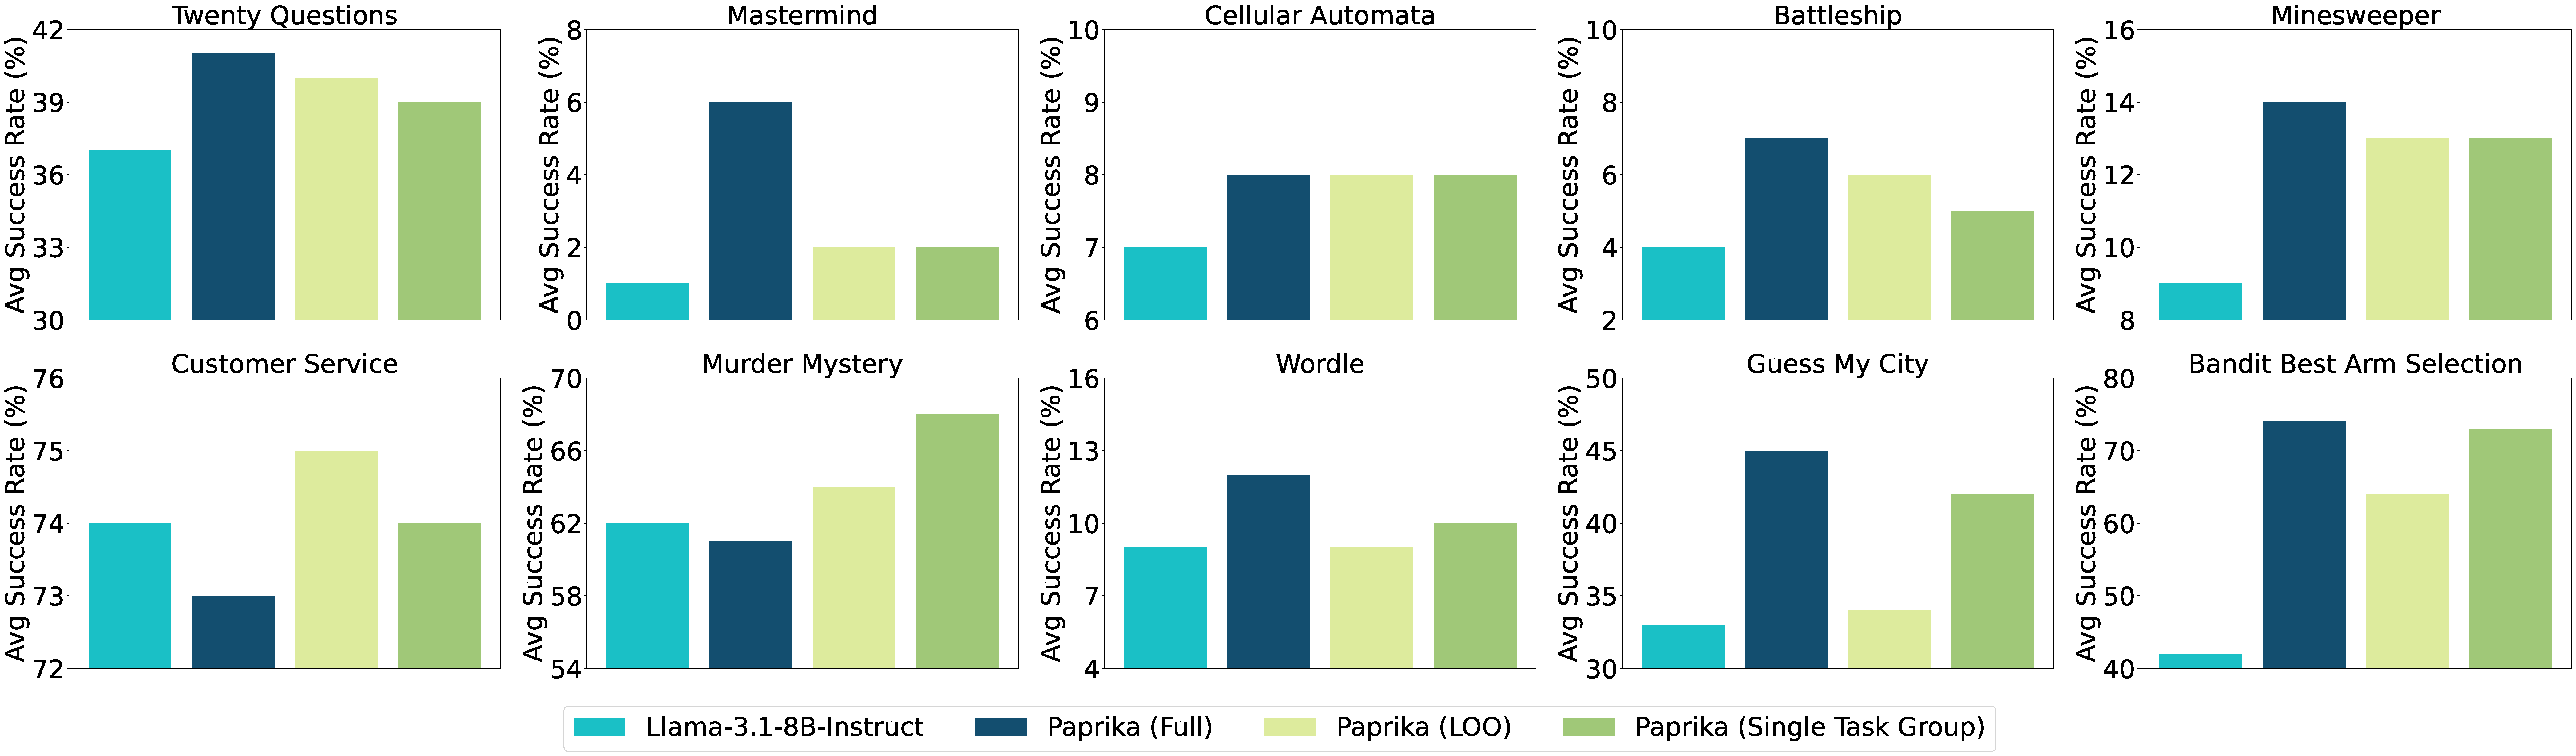
\includegraphics[width=0.95\linewidth]{figures/generalization.pdf}
    \Description{Bar chart comparing the initial model, leave-one-out training, single
    task group training, and full PAPRIKA on each task group.}
    \caption{\textbf{(Testing generalization of \textsc{PAPRIKA} via leave-one-out and
    single task group experiments)} 
    \textsc{PAPRIKA}'s zero-shot performance on unseen
    task groups is tested by leave-one-out (LOO) experiments, where the LLM is trained on
    every task group except the one it is tested on. \textsc{PAPRIKA} (Single Task Group)
    trains and tests the LLM on a single group. The learned decision making abilities
    often transfer well to new tasks without any additional training.}
    \label{fig:generalization_leave_one_out_experiments}
\end{figure}

\paragraph{Curriculum learning can improve data efficiency.}{
The biggest bottleneck of \textsc{PAPRIKA} is the time required to generate a large
number of trajectories, and harder tasks give smaller learning signal for an equal
sampling budget. To test the curriculum, GPT-4o-mini classifies the tasks in twenty
questions into 3 difficulty categories, resulting in 477 easy, 726 medium, and 296 hard
topics in the train split. The curriculum learning algorithm is run for 3 rounds on
Llama-3.1-8B-Instruct: at each round, 250 tasks are sampled from the train set according
to Algorithm~\ref{alg:sampling}, using the number of turns needed to solve a task as a
proxy for reward in Eq~\ref{eq:nu}. 20 trajectories are generated per task using the
previous round's checkpoint, which is then trained on the resulting dataset.
Figure~\ref{fig:curriculum} shows the results: after three rounds, the curriculum
outperforms uniform random sampling of tasks by 1.4\% and 3.3\% at average and pass@4
accuracy respectively.
}

%%% figure 4: curriculum learning on twenty questions %%%
\begin{figure}[t]
    \centering
    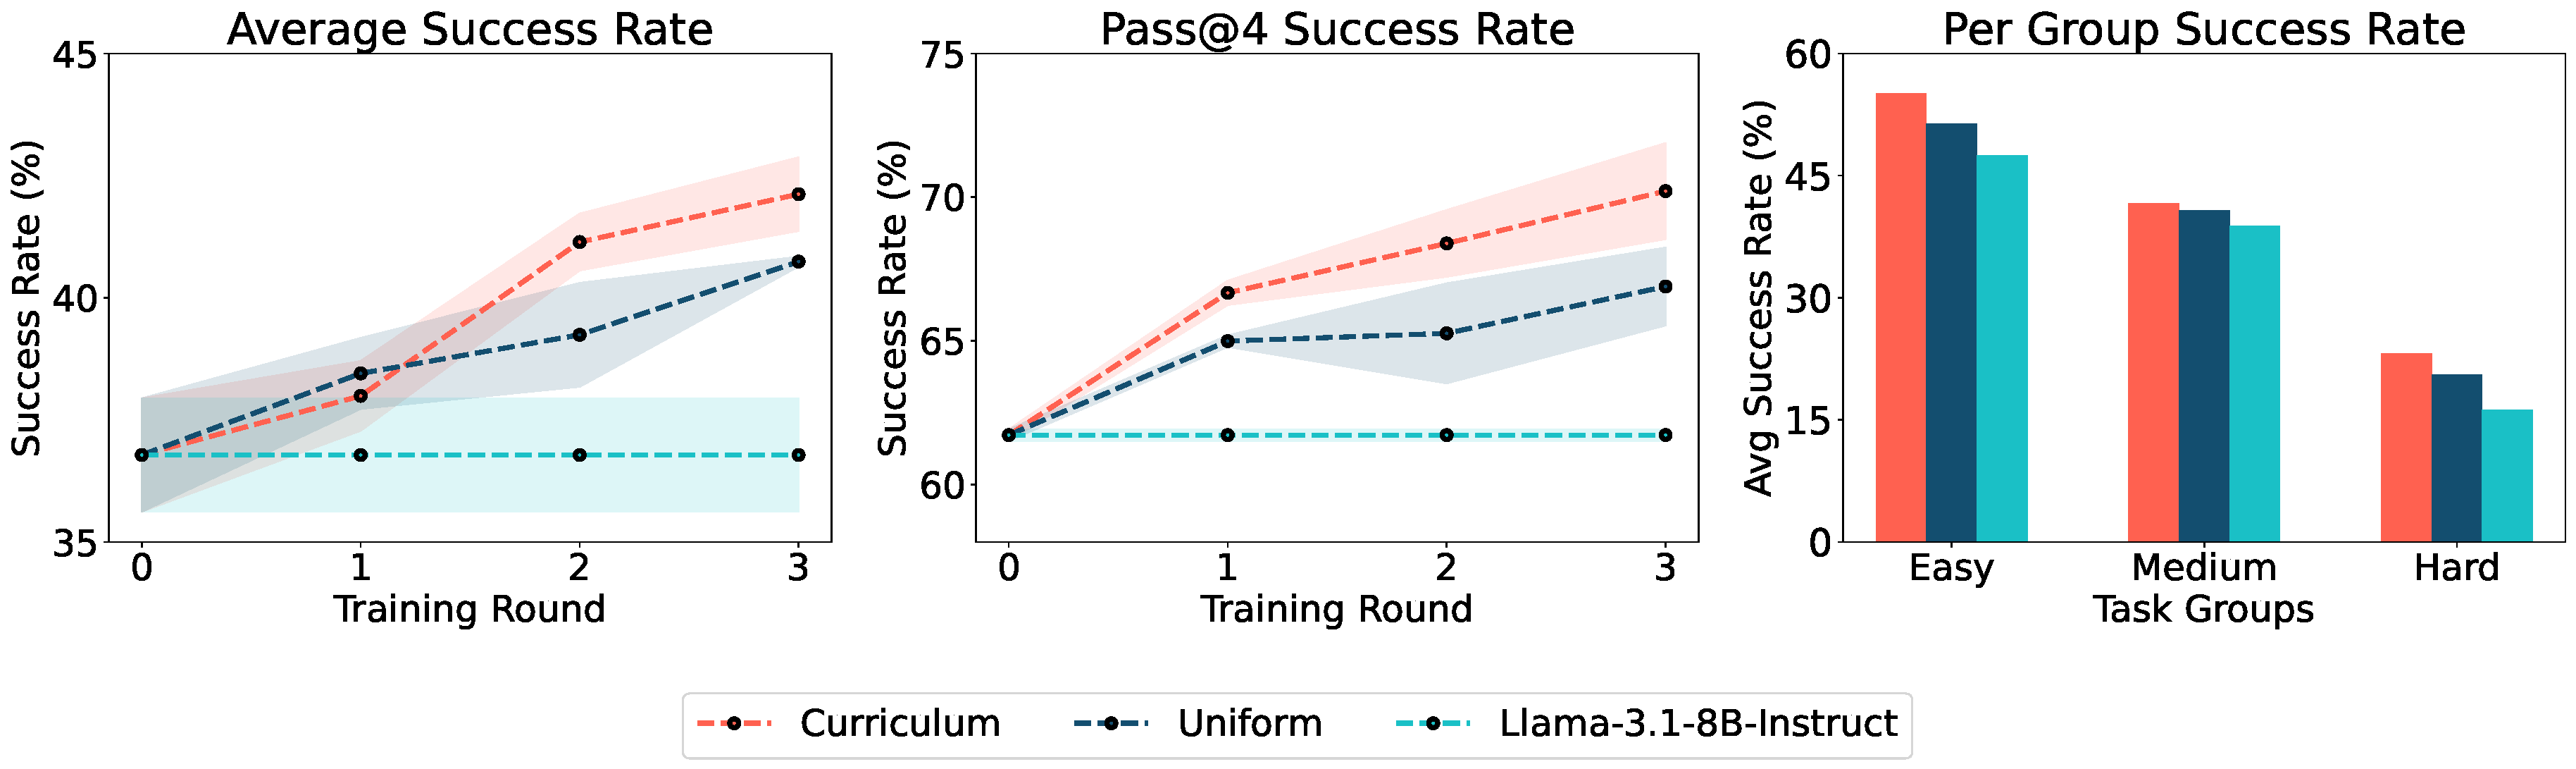
\includegraphics[width=0.95\linewidth]{figures/curriculum.pdf}
    \Description{Three line plots comparing curriculum learning against uniform sampling
    over three rounds of training on twenty questions.}
    \caption{\textbf{(Multi-round training with curriculum on twenty questions)}
    Performance of the curriculum learning algorithm against uniform sampling for
    multi-round training, with Llama-3.1-8B-Instruct as the initial model. (\textbf{Left})
    Average success rate at each round. (\textbf{Middle}) Pass@4 success rate at each
    round. (\textbf{Right}) Success rate per each of easy, medium, and hard task groups.}
    \label{fig:curriculum}
\end{figure}

\paragraph{\textsc{PAPRIKA} does not hurt LLMs' regular capabilities.}{
The tasks are designed so that an agent capable of better strategic exploration solves
them faster, and \textsc{PAPRIKA} indeed reduces the average number of turns it takes the
agent to solve tasks, implying that it chooses more optimal actions at intermediate
steps. Finally, since scaling up \textsc{PAPRIKA} should not come at the cost of the
model's general abilities, the fine-tuned model is compared against Llama-3.1-8B-Instruct
on a set of standard benchmarks. Table~\ref{tab:mt_bench_eval} shows the findings:
\textsc{PAPRIKA} does not result in any noticeable performance degradation.
}

%%% table 2: standard benchmark evals %%%
\begin{table}[t]
    \centering
    \caption{\textbf{(Evaluation of \textsc{PAPRIKA} on standard tasks)} Evaluation of
    \textsc{PAPRIKA} vs Llama-3.1-8B-Instruct on standard benchmarks (numbers in
    parenthesis represent standard error over 3 seeds). \textsc{PAPRIKA} does not result
    in significant model degradation.}
    \label{tab:mt_bench_eval}
    \begin{tabular}{c|cccccc}
        \toprule
        Model & MT-Bench & AlpacaEval & GPQA & Math (Hard) & MMLU-Pro & IFEval \\
        \midrule
         Llama-3.1-8B-Instruct  & 7.88                  & \textbf{33.6} & \textbf{33.5} & 24.6                  & \textbf{46.7} & 84.4\\
         + \textsc{PAPRIKA}     & \textbf{8.14 (0.03)}  & 33.5 (0.3)    & 32.8 (1.5)    & \textbf{25.3 (0.3)}   & 46.2 (0.1)    & \textbf{85.4 (0.3)} \\
         \bottomrule
    \end{tabular}
\end{table}
}
%%%%%%%%%%%%%%%%%%%%%%%%%%%%%%%%%%%%%%%%%%%%%%%%%%%%%%%%%%%%%%%%
\section{Discussion}
{
This paper presented a scalable fine-tuning method to improve the multi-turn decision
making abilities of LLMs, and showed that the strategies learned through it can
generalize zero-shot to unseen tasks. The approach has a few limitations. First, since
rejection sampling on self-generated data is used to teach the model better behaviors,
the starting model needs to exhibit good behavior within a reasonable generation budget,
so \textsc{PAPRIKA} would perform worse in the absence of a good base model. Second,
offline preference tuning algorithms were used due to the lack of computational
resources; running online RL on diverse tasks instead is a promising future direction
given its recent success in other
domains\cite{deepseekai2025deepseekr1incentivizingreasoningcapability}. Third, the
environments, despite being designed with the help of GPT-4o-mini, required a lot of
human effort to implement, training an LLM to scalably generate suitable tasks is a
new axis of improvement. Finally, the performance of the curriculum learning algorithm
depends heavily on the quality of the task group clusters, which leaves room for further
study. More broadly, this line of work can produce models with stronger strategic
exploration and decision making capabilities, and while the experiments here are
confined to relatively simple and controlled environments, it remains an open question
what kind of impact truly agentic systems will have on society.
}

%%% bibliography %%%
\bibliographystyle{unsrtnat}
\bibliography{refs}

\end{document}